\vspace{-.5cm}
\section{The Running Example: Quiz Controller}
\label{sec:example}
\vspace{-.2cm}
Our running example for this demonstration is a controller for a system that
allows playing quiz games -- Quiz Controller (QC) for short. The QC's function
is to turn on the light indicator of the player than presses the answer button
first. Three groups, more specifically 2 pupils, 1 high school student and 2
professors can play the game. There are 2 buttons for the pupils group, 1 button
for the high school student group and 2 buttons for the professors group. Such
that the pupils are favored, either of their buttons can be pressed to turn on
the indicator. Regarding the professors group, both their buttons need to
pressed simultaneously such the indicator is turned on. We directly illustrate
the behavior of the controller that we are building as a set of
\textsf{EARS-CTRL} requirements as shown in figure~\ref{fig:QC_reqs}.
Given \textsf{EARS-CTRL} is English, the requirements are self-explanatory.
\begin{figure*}[!h]
\centering
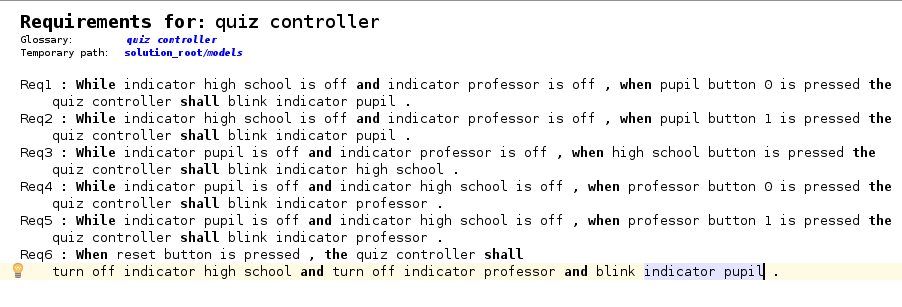
\includegraphics[width=1\textwidth]{./images/QC_Reqs.png}
\vspace{-1cm}
\caption{Requirements written in \textsf{EARS-CTRL} for a Quiz Controller}
\label{fig:QC_reqs}
\end{figure*}